\documentclass[]{article}

% Imports

\usepackage[utf8]{inputenc}
\usepackage{graphicx}
\usepackage[danish]{babel} %Benyttes til at oversætte abstract funktionen til dansk.

% Remove "New paragraph" indentation

\setlength{\parindent}{0cm}

% Meta info
\renewcommand{\contentsname}{Indholdsfortegnelse}
\selectlanguage{danish}


% Title Page
\title{Rapport}
\author{Martin Hansen \and Peter Christen Bloch}


\begin{document}

% Forsiden
\maketitle

\begin{figure}[h!]
	\centering
	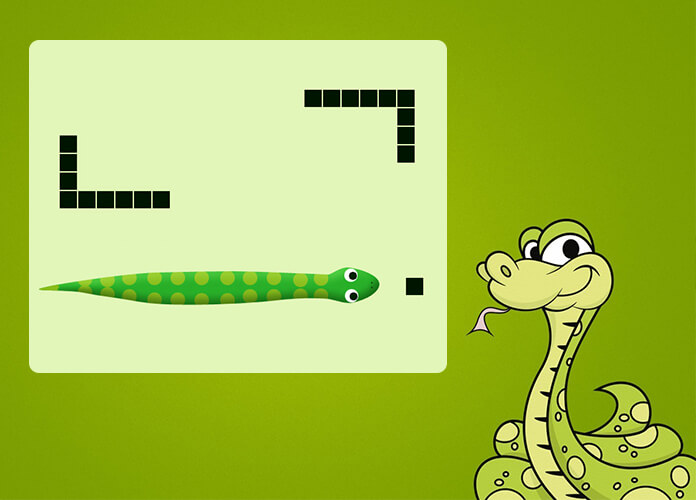
\includegraphics[width=\linewidth]{Snake_pic.jpg}
	\label{fig:diagram}
\end{figure}

\pagebreak % Forsiden stop

\begin{abstract}
	Resume
\end{abstract}

\pagebreak % Resume stop
\tableofcontents

\pagebreak
\section{Indledning}

Denne rapport indeholder en beskrivelse af de metoder og designvalg der førte til vores applikation \textit{Snake}. Dokumentet søger i grove træk at afdække programmets struktur og de overvejleser der lå til grund for denne og andre designtiltag. Derfor startes ud med en redegørelse for kravspecifikation og de tanker det automatisk vil medføre. Dernæst gøres der rede for den overordnede struktur i programmet med fokus på polyformi, design og implementation, og efterfølgende argumenteres der for de valg vi har taget undervejs i processen med henblik på en afsluttende vurdering af de udfordringer og problematikker der var under udarbejdelsen af \textit{Snake}. Afslutningsvist rundes af med en konklusion hvor kravspecifikation og endeligt resultat udmåles.

\section{Kravspecifikation og problemstilling}

Selve kravet til  vores applikation \textit{Snake}, er foruden de givne kravspecifikationer, at det i første omgang skal følge konceptet fra det klassiske Snake spil kendt fra den gamle mobiltelefon Nokia 3310. Dvs. en slange bevæger sig på en bane (en såkaldt \textit{torus}) og skal spise en madding i form af kollision mellem denne og slangen. Banens grænser er udefineret i den forstand at slangen aldrig helt forlader banen i det at ved udtræden via banens fire sider genindtrædes denne fra den modsatte side. Slangen bevæges ved hjælp af input fra brugeren i form af tastatur input hvor slangen rykkes et felt i ønsket retning. Banen består af et antal kolonner og rækker der fastsættes ved kommando linje parametre ved programmets opstart, og dette rejser så en problemstilling i forhold til de enkeltes felters geometriske design. Skal det være rektangler med parvis ens sidelængder eller kvadrater med ens sidelængder? Målet med vores applikation er muligheden for eksekvering på tværs af forskellige skærme, hvad enten det afvikles på en stationær computer med tilhørende full hd skærm eller en lille bærbar med en skærm ved standard hd opløsning\footnote{Her tænkes på opløsninger ved 1280x800 eller mindre.} og ydermere skabe en visual repræsentation af slangen der er hensigtsmæssig i en kosmetisk forstand.

\section{Ansvars fordeling}



\section{Struktur og rollefordelinger}

I den her sektion beskrives computerspillets polyformi og brug af nedarvning. Derudover redegøres der for de forskellige klassers roller og funktioner, og specielt brugen af threading omtales, da dette spiller en fundamental rolle i afviklingen af computerspillet Snake\footnote{Her refereres både til den simple variant, \textit{SimpleSnake}, og den mere avancerede del, \textit{AdvancedSnake}.}.
Selve spillet er opdelt i to dele, nærmere betegnet indeholder det to såkaldte pakker\footnote{En java package er et domæne bestående af et eller flere klasser og for dem med kendskab til c++ kan der henføres til namespace som benyttes til at kende forskel på de forskellige klasser I de tilfælde de deler samme navn.} , BaseKit og MainKit. Den første udgør spillets fundament, da de fleste klasser i pakken \textit{MainKit} er nedarvet fra klasser i \textit{BaseKit} og sørger for grundfunktionaliteten i programmet. Det vil omtales i detaljer i den næste sektion hvor der vil gås nærmere ind på de forskellige abstraktionslag i Snake med hensyn til indhold og anvendelse af dette, specielt i forhold til objekternes indbyrdes kommunikation. Den følgende illustration viser programmets polyformiske struktur inddelt i de to abstraktionsniveauer:

\begin{figure}[h!]
	\centering
	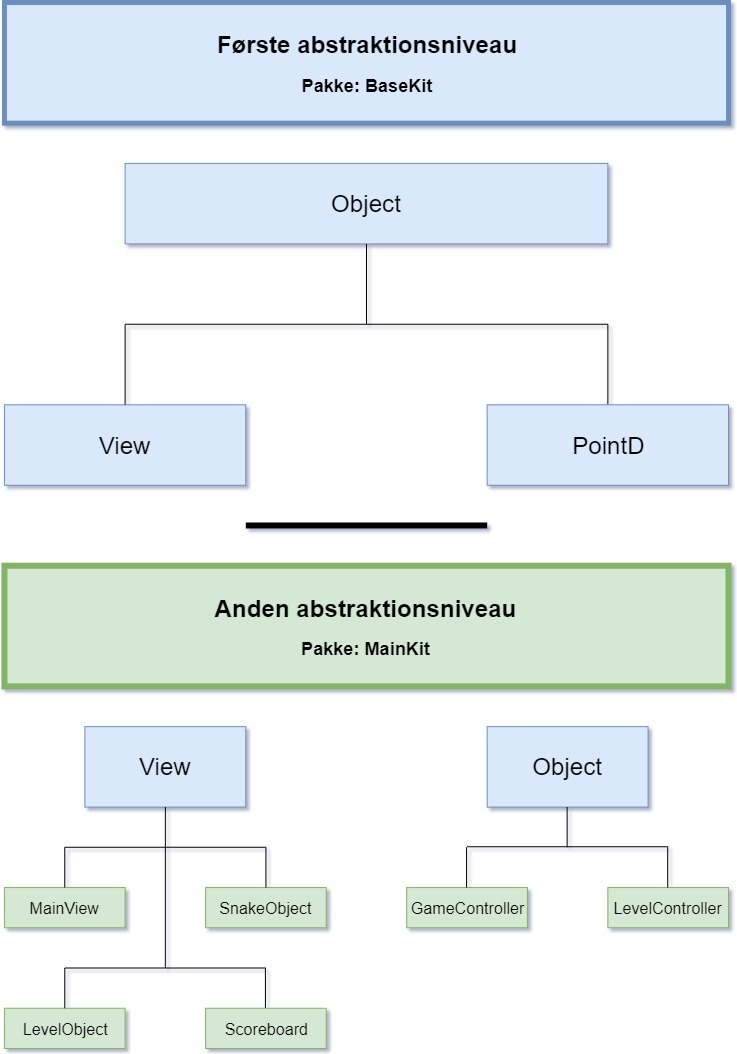
\includegraphics[width=200px]{Abstraktions_diagram.jpg}
	\label{fig:diagram}
\end{figure}

\subsection{Det indledende abstraktionsniveau}
Næsten alle klasser i Snake nedarver fra klassen \textit{Object} hvis primære funktion er at forsyne klasserne med meta information. På denne måde kan klasserne nemt findes ved hjælp af et koncept i denne rapport omtales som \textit{Parent and Child}. Dette koncept udgør en grundlæggende del af programmets struktur hvor objekter enten er \textit{children} af et objekt, eller et objekts \textit{parent}. Når et objekt tildeles parent status, tilføjes dens child til en liste af childrens som kan søges op senere hen i programmets forløb. Denne struktur er nyttig når der skal foretages callbacks i de tilfælde hvor klasser og objekter har behov for at udvekse information; f.eks. når klassen der repræsenterer slangen har behov for at sætte sine dimensioner eller Scoreboard skal opdateres.
Den klasse der implementerer \textit{Parent and Child} konceptet er \textit{View}, som er moderklassen for alle de objekter der visuelt repræsenteres på skærmen. Alle afledte klasser af denne klasse reimplementerer hver især \textit{draw()} som gør det enkelt og hurtigt at tegne en samling af objekter, hvad enten det er non-interaktive objekter som spillerflade og dens tilhørende objeker, eller semi-interaktive og interaktive objekter, som slangen eller maddingen\footnote{Med non-interaktive objekter menes der objekter der enten er fast inventar på spillerfladen eller objekter der ikke har direkte relation til objekter der agerer efter spiller input. Mål objektet som slangen skal opsluge er  dog ikke medtaget her men betegnes som et semi-interaktivt objekt da den har indvirkning på spiller objektet.}.  Derudover indeholder \textit{View} metoder og egenskaber der relaterer sig til objekters positioner på skærmen og dimensioner samt håndtering af brugerinput i form af interaktion via mus og tastatur. Det foregår ved hjælp af såkaldte eventhandlers som hver især kalder relevante metoder der kan reimplementeres af de afledte klasser. Den allervigtigste rolle View dog udfylder er opsætning og tegning af hele brugergrænsefladen\footnote{Her tænkes på alle visuelle objekter.}. Alle klasser der nedarver fra denne foretager et kald til metoden \textit{getPainter()} som returnerer et objekt af typen \textit{GraphicsContext} som kan betegnes som programmets malerpensel.
\subsection{Det andet, og primære, abstraktionsniveau}
Den første klasse der bliver instantiereret er klassen MainView, som udgør programmets visuelle del og fungerer som programmets hoved klasse. Det er denne klasse der håndterer de forskellige metode kald med hensyn til at tegne objekter eller håndtere input fra brugeren i form af keyboard input. En kort oversigt over strukturen indenfor domænet \textit{MainKit} kan illustereres i følgende figur:

\begin{figure}[h!]
	\centering
	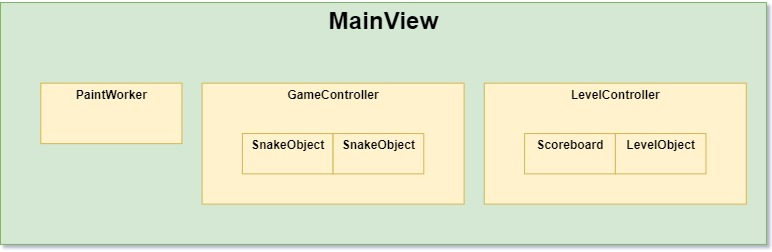
\includegraphics[width=200px]{Domain_diagram.jpg}
	\label{fig:diagram2}
\end{figure}

\subsubsection{Tegne delen}

MainView er klassen der sørger for at  tegne alle objekterne på grænsefladen i den reimplementerede metode \textit{draw()} som den får fra View klassen. Denne metode foretager et kald til de to controller klasser som hver især kalder deres respektive objekters \textit{draw()} metoder, da disse objekter alle er afledte af \textit{View}. Måden denne klasse bliver kaldt på foregår ved hjælp af klassen PaintWorker som er en såkaldt subclass af \textit{java.lang.Thread}\footnote{\textit{java.lang.Thread} er en klasse hvis metode \textit{run()} eksekverer kode i en separat tråd.}  og reimplementerer dens metode \textit{run()}. Alt kode i denne metode afvikles asynkront i en seperat tråd og dens formål er at opdaterer grænsefladen ved at foretage et kald til draw() metoden i MainView et bestemt antal gange i sekundet. Dette antal opdateringer kan så sættes til en bestemt værdi ved metoden \textit{setPollRate()}. Selve strukturen over de forskellige metodekald kan betragtes i følgende illustration:

\begin{figure}[h!]
	\centering
	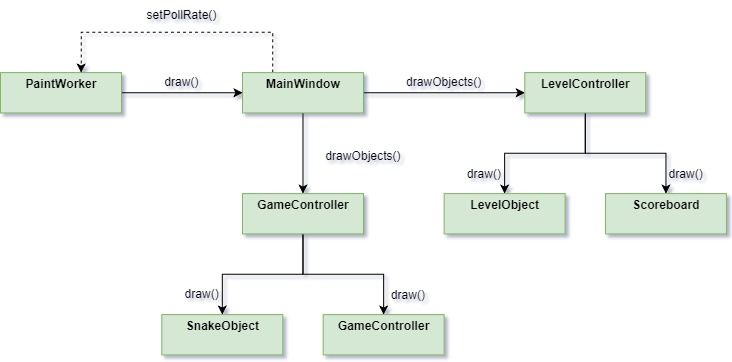
\includegraphics[width=250px]{Draw_sequence.jpg}
	\label{fig:diagram2}
\end{figure}

\subsubsection{Selve spillerfladens opbygning}

Selve spillerfladen består af et $r \times n$ gitter opdelt i kvadrater og tegnes i klassen \textit{LevelObject}. Banen optegnes ud fra nogle parametre som antallet af kolonner, rækker og grænsefladens dimensioner. Specielt dimensionerne på de kvadrater der udgør gitteret bestemmes relativt ud fra grænefladens højde, for på den måde at bibeholde en identisk skalering ved forskellige valg af rækker og kolonner. Dette tjener også som formål at sikre en uniform repræsentation ved forskellige skærmopløsninger. Dette omtales i et senere kapitel med henblik på de overvejelser der ligger til grund for dette valg.

\subsubsection{Håndtering af brugerinput}

Selve interaktionen foregår ved hjælp af tastatur input fra brugen hvorved denne danner basis for slangens bevægelser. Programmets gang styres enten af piletasterne eller andre taster, og kombinationer af modifikations tasterne og ordinære taster. Selve håndteringen af disse brugerinputs står klassen MainView for, der ved hjælp af metoden keyPressEvent(KeyEvent) videresender et \textit{javafx.scene.input.KeyCode}  objekt til GameController der derved på baggrund af den tast brugeren har trykket kalder de relevante metoder. Dette kan illustreres i nedenstående figur:


\begin{figure}[h!]
	\centering
	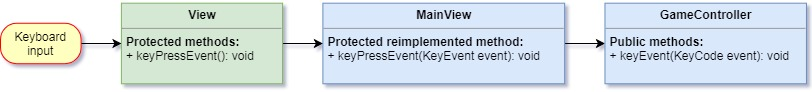
\includegraphics[width=\linewidth]{Event_sequence.jpg}
	\label{fig:Event}
\end{figure}

\textit{GameController} er klassen der styrer spillets gang og sørger for at håndtere kollisioner, opdatere slangens position og reinitialisere positionen når slangen befinder sig i grænseområderne. Det sidste foregår ved hjælp af det førnævnte \textit{Parent and Child} koncept, hvor \textit{GameController} foretager et metodekald til en af sine nedarvede metoder \textit{object(String)} der ud fra den tildelte meta information, returnere selve baneobjektet \textit{LevelObjekt}. Dette baneobjekt tildeler slangen, som repræsenteres af klassen \textit{SnakeObjekt}, sine dimensioner som den får fra metoden \textit{BlockSize()}.\\

\section{Brugen af seperate tråde, og ideén bag det}

Ideén bag brugen af en seperat tråd til automatisk optegning af grænsefladen, bunder i en tanke om kun at skulle opdatere de enkelte semi- og interaktive objekters positioner på spillerfladen uden brug af kald til deres respektive \textit{draw()} metoder. 	 

\end{document}          
